\documentclass[12pt,a4paper]{article}

\input{/home/tabaka/Documents/GitHub/Defs/defs.tex}

\setcounter{zadaniaRozdzial}{3}

\begin{document}
	
	\begin{center}
		\LARGE Karta 3
	\end{center}
	\vspace{1.5cm}
	
	\ZbiorZadanie{
		Punkty $A,B,D$ należą do okręgu o środku w punkcie $O$. Sieczne $AB$ i $DO$ przecinają się w punkcie $C$ (zobacz rysunek). Wykaż, że jeśli $|BC| = |BO|$, to $|\angle DOA| = 3|\angle COB|$.
		
		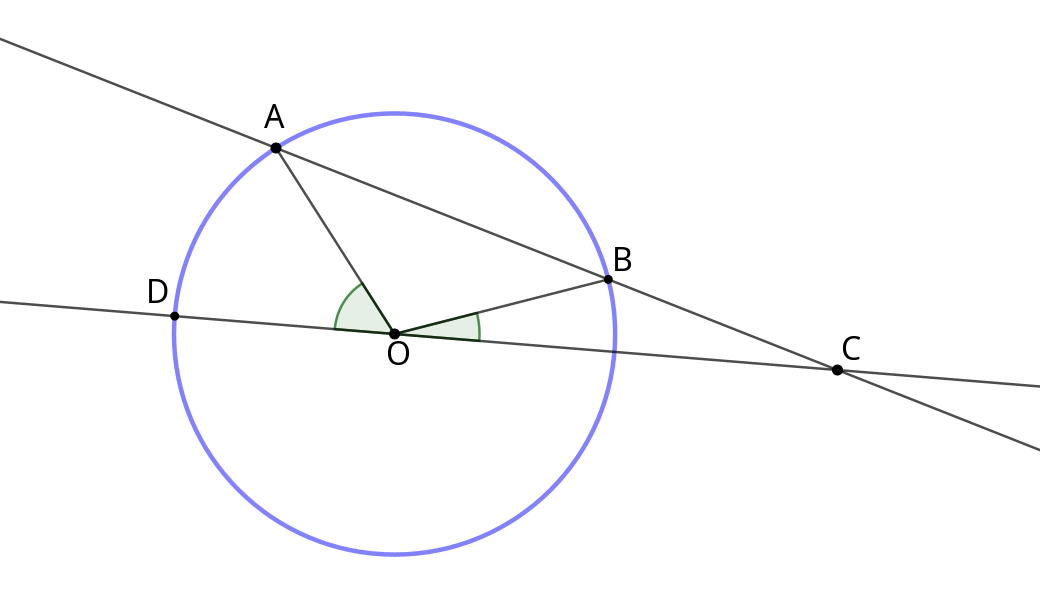
\includegraphics[width=13cm]{K3_1}
	}
	
	\ZbiorZadanie{
		Dwa okręgi o środkach $O_1$ i $O_2$ i różnych promieniach przecinają się w punktach $A$ i $B$. Przez punkt $B$ poprowadzono sieczną prostopadłą do cięciwy $AB$, która przecięła te okręgi odpowiednio w punktach $C$ i $D$. Wykaż, że $|CD|=2|O_1O_2|$.
	}
	
	\ZbiorZadanie{
		Wykaż, że jeśli równanie
		$$x^3+bx^2+2bx+8=0$$
		ma dwa różne rozwiązania, to $b=-2$.
	}
	
	\ZbiorZadanie{
		Wielomian $W(x)=x^4+ax^3+bx^2-24x+9$ jest kwadratem wielomianu $P(x)=x^2+cx+d$. Oblicz $a$ oraz $b$.
	}
	
	\ZbiorZadanie{
		Kąt $\alpha$ jest taki, że
		$$\cos\alpha + \sin\alpha = \frac{4}{3}.$$
		Oblicz wartość wyrażenia $|\cos\alpha - \sin\alpha|$.
	}
	
	\ZbiorZadanie{
		Wyznacz wszystkie wartości parametru $m$, dla których równanie
		$$2x^2 + (3-2m)x -m + 1 =0$$
		ma dwa różne pierwiastki $x_1,x_2$ takie, że $|x_1-x_2|=3$.
	}
	
	\newpage
	
	\setcounter{zadaniaIndex}{0}
	
	\ZbiorZadanie{Odpowiedź wynika bezpośrednio z tezy. Wystaczy rozpisać kąty.}
	
	\ZbiorZadanie{Wystarczy zauważyć, że mamy kąt prosty $\Rightarrow$ trójkąt prostokątny, którego środek przeciwprostokątnej leży w środku okręgu $\Rightarrow$ trójkąty są podobne.}
	
	\ZbiorZadanie{
		$x=-2$ jest zawsze miejscem zerowym. Następnie stosujemy schemat Hornera i rozważamy przypadki dla funkcji kwadratowej.
		
		I. $\Delta=0$.
		
		II. $-2$ jest rozwiązaniem i istnieje jeszcze inne rozwiązanie.
		
		Z pierwszego przypadku dostajemy $b=-2$ lub $b=6$, ale w drugim przypadku również dostajemy $b=6$, czyli mielibyśmy jedno rozwiązanie trzykrotne. Zatem $b=-2$.
	}
	
	\ZbiorZadanie{
		$\UkladRownan{a=-8}{b=22}$
		lub
		$\UkladRownan{a=8}{b=10}$.
	}
	
	\ZbiorZadanie{
		$|\sin\alpha-\cos\alpha|=\frac{\sqrt{2}}{3}$.
	}
	
	\ZbiorZadanie{
		I. $\Delta>0 \Rightarrow m\neq-\frac{1}{2}$.
		
		II. $m=-2\frac{1}{2}\vee m=3\frac{1}{2}$.
	}
	
\end{document}